%!TEX root = index.tex
\chapter[Revisão Bibliográfica]{Revisão Bibliográfica}
\label{chap:revisao}

Nesse Capítulo serão apresentados os principais conceitos usados no desenvolvimento do método e na resolução do problema apresentado.

O Capítulo será dividido em dois grandes blocos: Startup Enxuta e Estratégia.

O bloco Startup Enxuta irá focar nos conceitos de administração de startups. Serão apresentadas as propostas de Steven Blank e Bob Dorf sobre o Desenvolvimento de Clientes. Além disso serão abordadas as propostas de Eric Ries sobre elaboração de hipóteses e testes para buscar a Aprendizagem Validada.

Já o bloco Estratégia focará no conceito de Canvas de Modelo de Negócio, Canvas de Proposição de Valor e em alguns pontos importantes de Peter Thiel.

\section{Startup Enxuta}
\label{cha:startupenxuta}
As revisões bibliográficas contidas nesse bloco irão focar nos principais conceitos da Startup Enxuta. \citeonline{leanstartup} define uma startup da seguinte maneira: "Uma startup é uma instituição humana projetada para criar novos produtos e serviços sob condições de extrema incerteza." (RIES, 2011, p. 24). \citeonline{leanstartup} afirma que a Startup Enxuta é um conjunto de práticas para aumentar as possibilidades de sucesso de uma startup. Tais práticas foram baseadas no sistema de manufatura enxuta que nasceu no Japão com o Sistema de Produção Toyota idealizado por Taiichi Ohno e Shigeo Shingo.

\subsection{O método da Startup Enxuta}
\label{cha:metodostartupenxuta}
As startups são empresas inovadoras, disruptivas e caóticas e apesar disso elas necessitam de gestão, afirma \citeonline{leanstartup}. Muitas startups fracassam por tentarem aplicar metodologias antigas de administração que focam em um bom planejamento, estratégia sólida e uma pesquisa de mercado completa. Entretanto, segundo \citeonline{leanstartup}, planejamento e previsão só são precisos quando se tem um histórico operacional longo e estável oque não se aplica no meio no qual as startups estão imersas. Outras startups fracassam por adotarem a prática de "simplesmente faça" e repudiarem qualquer tipo de gestão.

O método da Startup Enxuta é divido em três partes: "Visão", "Direção" e "Aceleração". Entretanto, serão abordados só as duas primeiras nessa revisão bibliográfica dada que a terceira parte se aplica a startups que já possuem grande parte de suas hipóteses validadas.

Na parte "Visão", \citeonline{leanstartup} introduz o conceito da aprendizagem validada que é uma maneira de medir se as startups estão progredindo. Na parte "Direção", encontram-se os importantes conceitos do ciclo básico de feedback Contruir-Medir-Aprender e da contabilidade para inovação.


\subsubsection{Aprendizado Validado}
\label{cha:apredizado_validado}
\citeonline{leanstartup} afirma que uma startup não existe apenas para fabricar coisas e ganhar dinheiro. A função dela é aprender a criar um negócio sustentável e que isso poderá ser validado cientificamente por meio de experimentações frequentes. E assim como na manufatura enxuta, o aprendizado de onde e quando investir recursos resulta em economia de tempo e dinheiro.

Um empresa nascente tem como objetivo descobrir o que deve criar, algo que os seus clientes aceitem pagar, o mais rápido possível. Segundo \citeonline{leanstartup}, aprendizagem validada é o processo de demonstrar de modo empírico que um time fez descobertas de valor sobre as perspectivas de negócios presentes e futuros de uma startup.

O aprendizado validado é respaldado por dados de clientes reais pois implica na melhora dos indicadores chave da empresa nascente. Para a startup ser produtiva ela deve buscar sistematicamente as coisas certas para serem desenvolvidas. Ao invés de gastar tempo pensando se o produto pode ser desenvolvido, a empresa deve se perguntar se ela deve desenvolver tal produto ou tal serviço, e além disso, deve se perguntar se é possível desenvolver um negócio sustentável em torno desses produtos e serviços. \cite{leanstartup}

Deste modo, \citeonline{leanstartup}, recomenda que cada funcionalidade, produto e campanha publicitária sejam tratados como se fossem um experimento científico para alcançar a aprendizagem validada.

Com a aprendizagem validada sendo executada com sucesso a startup escapa de um grande problema: gastar tempo e recursos preciosos para construir algo que ninguém quer.

\subsubsection{Experimentação da Startup}
\label{cha:experimentacao_da_startup}

\citeonline{leanstartup} afirma que uma das lições mais importantes do método científico é que para aprender você deve poder fracassar. O objetivo de todo experimento associado à empresa nascente é descobrir como desenvolver um negócio sustentável em torno da visão \cite{leanstartup}.

O modelo da startup enxuta confere um método rápido para testar as hipóteses que permeiam a visão da empresa de modo a mitigar desperdícios ao longo do caminho.

Tal método tem como primeiro passo dividir a visão em partes menores. Segundo \citeonline{leanstartup}, as hipóteses de valor e de crescimento são as duas suposições mais importantes para os empreendedores.

A hipótese de valor tem como objetivo testar se o produto ou serviço deveras fornece valor para os clientes no momento em que estão o usufruindo. Por outro lado, a hipótese de crescimento tem em sua concepção testar como os novos clientes irão achar um produto ou serviço. \cite{leanstartup}.

\citeonline{leanstartup}, afirma que o experimento deve ser encarado com um primeiro produto ao invés de uma simples pesquisa teórica. Tais experimentos/produtos irão variar em sua complexidade de modo a garantir a aprendizagem validada.

\subsubsection{Ciclo de Feedback Construir-Medir-Aprender}
\label{cha:ciclo_cma}

O ciclo de feedback construir-Medir-Aprender está no centro da startup enxuta. Segundo \citeonline{leanstartup}, a atividade fundamental de uma startup é transformar ideias em produtos e/ou serviços, medir como os clientes reagem às iterações deles e depois aprender se é necessária a pivotação ou se é possível perseverar na mesma direção. Todos os processos da startup devem ter como norte percorrer esse ciclo o mais rápido possível.

O planejamento de como percorrer o ciclo Construir-Medir-Aprender deve ser feito na ordem inversa. Primeiro, deve-se pensar qual aprendizado o experimento está buscando. Posteriormente deve-se planejar quais medições serão realizadas a fim de se determinar se houve de fato uma aprendizagem validada. Só no final deve-se pensar qual produto será desenvolvido com a finalidade de executar o experimento e obter tais medições. \cite{leanstartup}

\begin{figure}[H]
\caption{Ciclo de Feedback Construir-Medir-Aprender}
\centerline{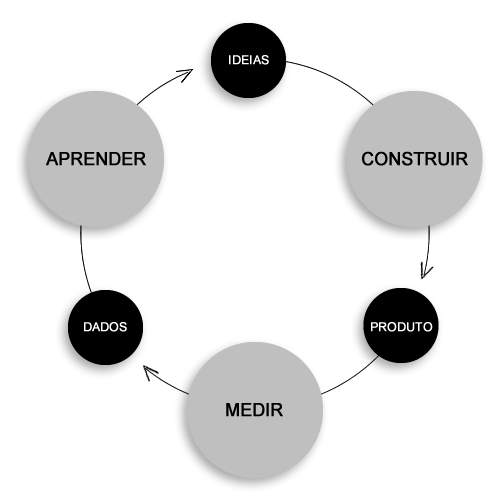
\includegraphics[scale=0.5]{img/ciclo_construir_medir_aprender}}
\label{fig:ciclo_construir_medir_aprender}
\caption* {Fonte: \citeonline{leanstartup}}
\end{figure}

\subsubsection{Atos de fé}
\label{cha:atos_de_fe}

\citeonline{leanstartup} afirma que o papel da estratégia nas startups é descobrir as perguntas certas para se fazer. O primeiro desafio de um empreendedor é transformar a sua empresa em uma máquina de testes para responder tais perguntas sistematicamente. O segundo desafio é continuar conduzindo testes rigorosamente sem perder de vista a visão geral da empresa.

Todo plano de negócios começa com uma série de hipóteses. O plano traça uma estratégia que considera essas hipóteses verdadeiras e prossegue mostrando como alcançar a visão da empresa. \citeonline{leanstartup} chama as suposições mais importantes de atos de fé, porque todo o sucesso do empreendimento depende da veracidade de tais hipóteses. Se elas se provarem verdadeiras, um grande sucesso acontecerá. Caso contrário a startup pode estar fadada ao fracasso.

\citeonline{leanstartup} ressalta a importância do conceito \textit {Genchi Gembutsu} (vá e veja por si mesmo) da manufatura enxuta. Tal expressão japonesa implica na relevância de basear decisões estratégicas na compreensão direta de seus clientes. Os dados dos clientes que devem ser recolhidos só existem fora do escritório.

\subsubsection{Testes}
\label{cha:testes}

Na parte Construir do ciclo Construir-Medir-Aprender o método da startup enxuta prega o emprego do conceito do MVP que é a sigla em inglês para Minimum Viable Product, cujo significado é Produto Mínimo Viável.

Segundo \citeonline{leanstartup}, o MVP tem como finalidade ajudar os empreendedores a começar o processo de aprendizagem o mais rápido possível tendo o objetivo de testar hipóteses fundamentais do negócio. Ele é apenas o primeiro passo na grande jornada em busca do aprendizado validado, após um certo número de iterações o empreendedor pode descobrir que sua estratégia era falha e pode decidir mudar de rumo para tentar reconquistar sua visão.

\begin{figure}[H]
\caption{Visão da Startup}
\centerline{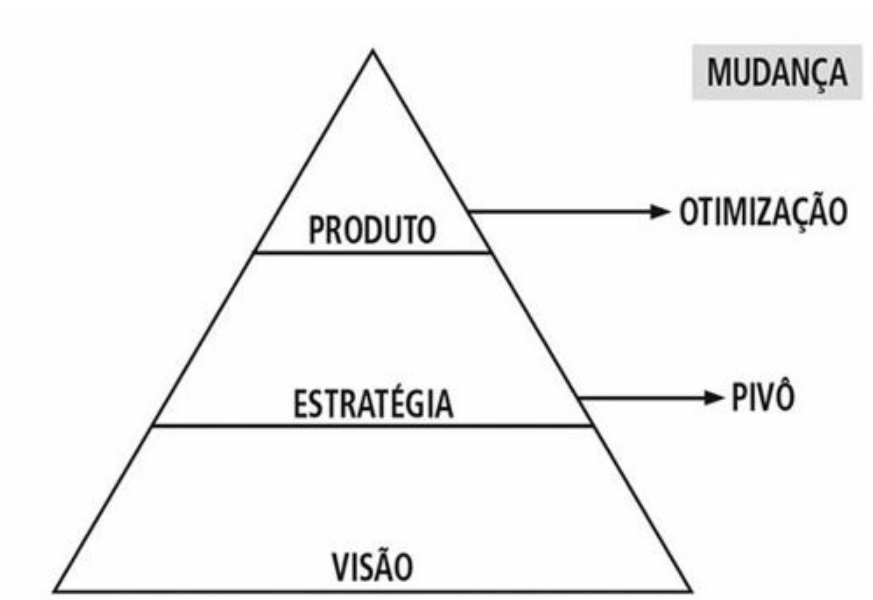
\includegraphics[scale=0.2]{img/pivotar}}
\label{fig:pivotar}
\caption* {Fonte: \citeonline{leanstartup}}
\end{figure}

A lição do MVP é que qualquer trabalho adicional além do requerido para iniciar o ciclo de aprendizagem é considerado desperdício. O empreendedor deve se lembrar

que mesmo um MVP de baixa qualidade pode estar atuando em prol de um grande produto de qualidade de ponta. E que enquanto não souber quem é o cliente, o empreendedor jamais saberá o que é qualidade. \cite{leanstartup}

\citeonline{leanstartup}, também cita os conceitos dos adotantes iniciais e de feedback constante. Os adotantes iniciais devem ser os primeiros clientes, pois eles se importam mais com o fato de serem os primeiros a utilizar um produto novo e são mais indulgentes com falhas de projeto do que os clientes normais. O feedback constante baseia-se em sempre ter clientes para testar protótipos para a melhoria contínua em cima das iterações do produto.

\subsubsection{Medir}
\label{cha:medir}

Em seus primeiros momentos a startup apenas admira os belos números estimados no plano de negócios. \citeonline{leanstartup} propõe duas tarefas para a startup. A primeira é medir rigorosamente onde ela está naquele momento (baseline). A segunda é iterar através de experiências para mover os números para cima buscando atingir a meta idealizada no plano de negócios.

Muitas empresas enfrentam dificuldades para saber se as mudanças feitas nos produtos trouxeram algum resultado tanto para melhor ou pior. Outra dificuldade é saber se foram extraídas as lições corretas dessas mudanças. \citeonline{leanstartup} então propõe o modelo da contabilidade para inovação, sua principal finalidade é tornar os saltos de fé em modelos financeiros quantificados. O modelo funciona em três etapas:
\begin{enumerate}
\item Utilizar um MVP para adquirir dados reais e determinar onde a empresa se encontra no momento.
\item Iterar através de experimentos para tentar melhorar os números de forma a alcançar o plano.
\item Depois de um certo número de iterações de forma a melhorar o produto a startup deve decidir se é hora de pivotar, mudar a estratégia, ou se deve insistir na mesma estratégia.
\end{enumerate}

Segundo \citeonline{leanstartup}, a análise de coorte é uma das ferramentas mais importantes ao analisar uma startup. Ao invés de olhar para números acumulados ou números brutos como receita total e número total de usuários, o autor propõe que a startup considere o desempenho de cada grupo de clientes que entra em contato com o produto independentemente. Cada grupo é chamado de coorte.

A análise de coorte é de extrema utilidade em diversas variedades de negócios, porque para sobreviver cada empresa é dependente de sequências de comportamentos de clientes denominadas fluxos. Esses fluxos de clientes irão determinar a interação dos clientes com os produtos de uma empresa, isso permitirá a compreensão de um negócio em termos quantitativos e apresentarão um poder de previsão muito melhor do que a métrica bruta tradicional. \cite{leanstartup}

\subsection{Desenvolvimento de Clientes}
\label{cha:desenvolvimento_de_clientes}
Muitas startups surgem de uma ideia, propõem uma solução e definem seu plano de negócios baseado em hipóteses que elas possuem em relação ao mundo. Mas nem sempre as suas hipóteses são as melhores, e por falta de testes dessas hipóteses elas acabam descobrindo seu erro somente no lançamento do produto perante o mercado.

Segundo \citeonline{startupowners}, o modelo de desenvolvimento de produtos é um dos principais culpados pelo fracasso de muitas startups. Muitas startups da época da bolha das ponto-com tinham como  em comum que o seu maior componente de risco era o de mercado, não o tecnológico. \citeonline{startupowners} explica os problemas que há nesta abordagem. São muitas as explicações que \citeonline{startupowners} utiliza para justificar esses problemas. Uma das explicações é que muitas empresas nascentes focam na execução e não no aprendizado. A startup mesmo tendo ciência de que existem várias suposições que ainda não foram testadas, usufrui do plano de negócios para acompanhar a execução. Outro motivo é o fato de que grande parte dos empreendedores acabam criando uma cultura baseada em politicagem. Ou seja, as suposições são criadas baseadas em opiniões ao invés de fatos e para piorar não existe uma preocupação na validação destas hipóteses.

A metodologia de desenvolvimento de clientes proposta por \citeonline{startupowners} tem como premissa que tudo que envolve o problema e a solução que englobam o produto/serviço são apenas suposições que necessitam ser testadas, validadas e renovadas. Portanto, após uma validação mercadológica, há a possibilidade que a premissa feita no começo seja transformada por completo. A metodologia proposta por \citeonline{startupowners} defende um processo iterativo feito paralelamente ao desenvolvimento do produto, criando um modelo de negócios que atende cada vez mais as necessidades reais do cliente, o que faz diminuir o risco do produto ser refutado no mercado.

\citeonline{startupowners} propôs um modelo de desenvolvimento de clientes que é dividido em quatro etapas que serão detalhadas abaixo:
\begin{enumerate}
\item Descoberta do cliente.
\item Validação do cliente.
\item Criação do cliente.
\item Construção da Empresa
\end{enumerate}

\begin{figure}[H]
\caption{Processo de desenvolvimento de clientes}
\centerline{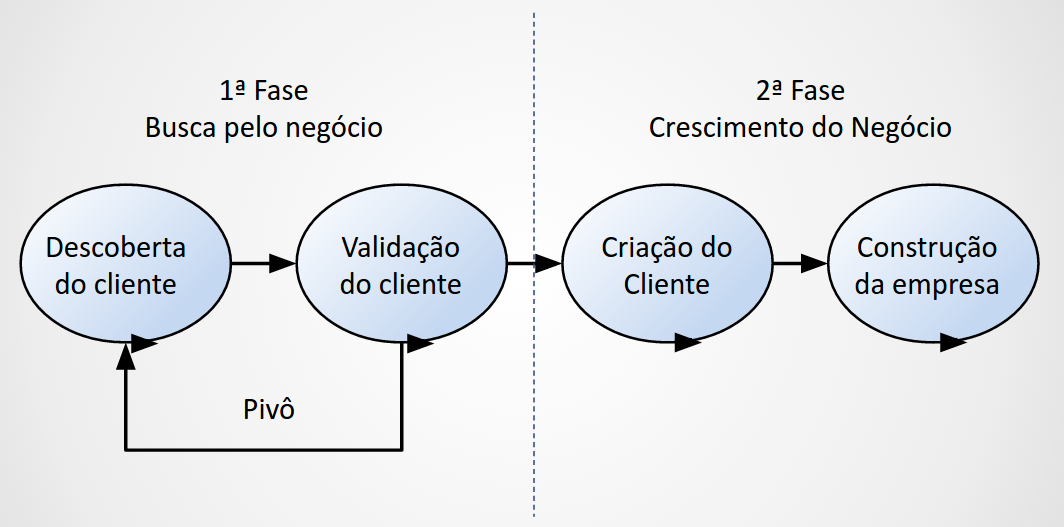
\includegraphics[scale=0.75]{img/desenvolvimento_de_clientes}}
\label{fig:desenvolvimento_de_clientes}
\caption* {Fonte: \citeonline{startupowners}}
\end{figure}

\subsubsection{Descoberta do cliente}
\label{cha:descoberta_do_cliente}
\citeonline{startupowners} descrevem nesta etapa como a empresa nascente deve descobrir o encaixe entre o problema e a solução.
\citeonline{startupowners} defendem a premissa de parar de vender e começar a ouvir. Dentro da empresa não há fatos, apenas opiniões, politicagem. Para descobrir os fatos, o empreendedor deve ir a rua, sair do escritório e da sua zona de conforto.
Outro item que \citeonline{startupowners} defendem é o teste de hipóteses. Duas suposições fundamentais que precisam ser testadas são: 
\begin{itemize}
\item Concepção do problema
\item Concepção do produto
\end{itemize}

Segundo \citeonline{startupowners}, o empreendedor deve entender quais são os problemas mais relevantes do cliente e verificar se o produto que a startup desenvolveu de fato resolve tais problemas. É de fundamental importância saber se o cliente concorda com a solução elaborada e mais ainda se eles estarão dispostos a pagar pelo produto/serviço desenvolvido. É nesta etapa que a empresa precisa gastar boa parte do tempo para decifrar quem é o cliente, quais são as suas necessidades, quais serão os custos, recursos gastos nesse projeto, quem são os concorrentes, entre outros pontos. Essa etapa é um ciclo, que só deve ser considerado acabado quando a startup estiver crente que o produto desenvolvido de fato é uma solução para o problema de alguma pessoa.

\begin{figure}[H]
\caption{Descoberta do Cliente}
\centerline{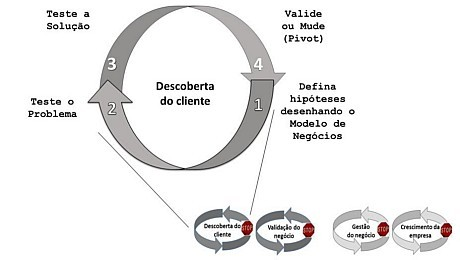
\includegraphics[scale=0.75]{img/descoberta_do_cliente}}
\label{fig:descoberta_do_cliente}
\caption* {Fonte: \citeonline{startupowners}}
\end{figure}

\citeonline{startupowners} afirmam que para \textit{websites} e para aplicativos a descoberta do cliente começa quando a primeira versão desse \textit{website} ou aplicativo está no ar. Assim os empreendedores já conseguem testar suas hipóteses baseados nesse produto mínimo viável e ajustar as estratégias de aquisição de clientes iterativamente. Tal tática foi utilizada por empresas como Facebook e Groupon que começaram a jornada por busca de clients com produtos mal acabados.

\subsubsection{Validação do cliente}
\label{cha:validacao_do_cliente}
O processo de validação do cliente, descrito por \citeonline{startupowners}, é a segunda fase do processo de desenvolvimento de clientes e oferece aos empreendedores uma forma de projetar os aprendizados requisitados para o desenvolvimento de seu modelo de negócio. 

Nesta etapa, \citeonline{startupowners} afirmam que a seguinte pergunta deve ser solucionada: Os clientes irão pagar pelo seu produto/serviço? A startup precisa entender como funciona o modelo financeiro da empresa bem como o seu cicl de vendas. O processo comercial e de logística do produto devem ser validados. Essa fase tem como objetivo encontrar um modelo de vendas escalável e adaptável e por fim validá-lo. 

Segundo \citeonline{startupowners}, a Validação do Cliente é uma maneira que permite desenvolver um processo de vendas. A etapa de validação tem como finalidade provar que a empresa nascente encontrou uma série de clientes que gostaram do produto e que há de fato um mercado. É uma etapa que validará o processo de marketing e comercial, onde tudo poderá ser modificado, inclusive o cliente. Se esse fato ocorrer, deve-se voltar para a fase de Descoberta do Cliente onde um novo tipo de cliente será análisado. Tal retorno é conhecido como Pivô. Essa etapa também é um ciclo de melhora e adaptação do modelo de negócios.

\begin{figure}[H]
\caption{Validação do Cliente}
\centerline{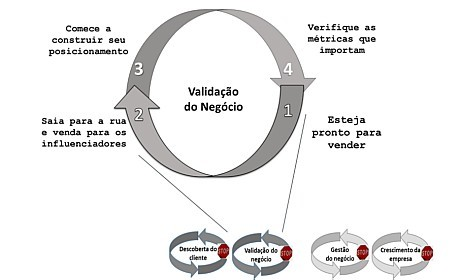
\includegraphics[scale=0.75]{img/validacao_do_cliente}}
\label{fig:validacao_do_cliente}
\caption* {Fonte: \citeonline{startupowners}}
\end{figure}

\subsubsection{Criação do cliente}
\label{cha:criacao_do_cliente}
Segundo, \citeonline{startupowners}, nesse momento busca-se uma maior demanda para a área comercial. Nessa etapa que se torna importante a definição de quais mercados a startup irá atuar, bem como a busca por uma quantia maior de investimento caso necessário. Será necessário definir bem os mercados, além de analisar a concorrência e os riscos que serão tomados. É a etapa onde será feito o marketing do produto, portanto, será necessário escalar tanto a área de vendas quanto a área de marketing.

\subsubsection{Construção da empresa}
\label{cha:construcao_da_empresa}
\citeonline{startupowners} afirmam que esta fase é o fim da transição entre uma empresa que foca em aprender para uma que foca em executar. Nesta etapa, a organização enfrentará novos desafios como o de crescer e atingir as massas. Enquanto a empresa cresce ela também deve evoluir quanto as suas estratégias de de gerenciamento.

\subsection{Métricas Pirata para Startups}
\label{cha:metricas_pirata}
\citeonline{mcclure2007startup} propõe um método para mapear o ciclo de vida de clientes que ficou famoso pelo nome de Métricas Pirata para Startups que possui cinco passos: Aquisição, Ativação, Retenção, Recomendação e Receita, como se fosse um funil como mostra a \autoref{fig:metricas_pirata}. Esses passos formam o acrônimo "AARRR", que parece com o som de um pirata, por isso o nome métricas pirata.
O método é utilizado mais regularmente por empresas que possuem uma interface web ou móvel, tais como sites e aplicativos.

\begin{figure}[H]
\caption{Métricas Pirata para Startups}
\centerline{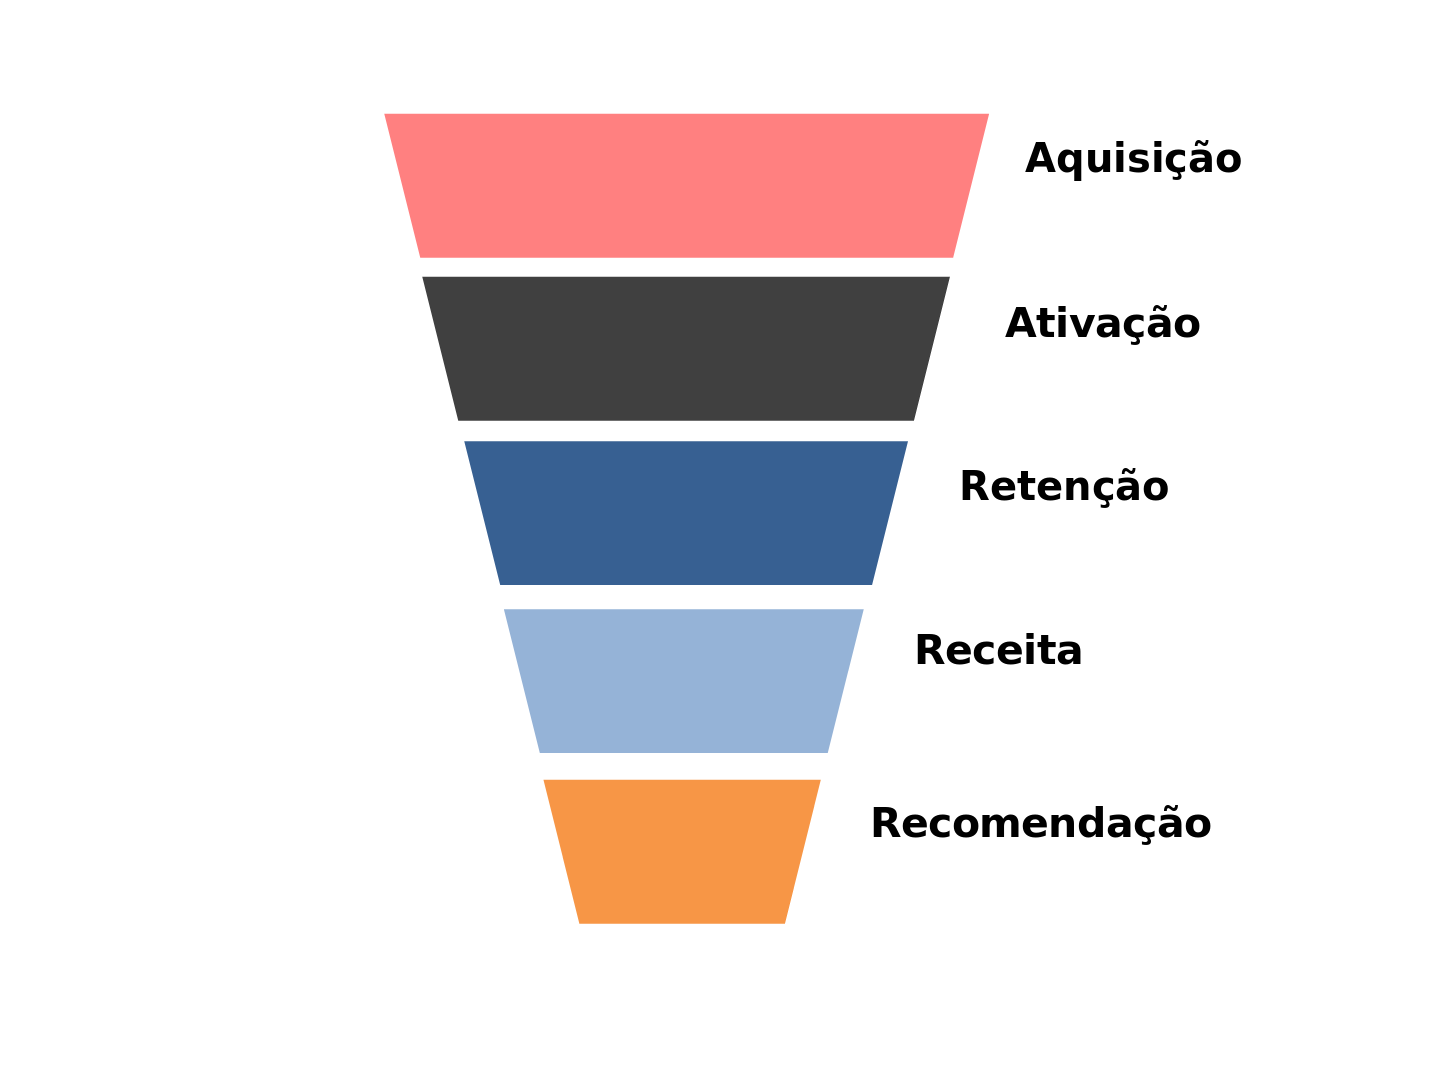
\includegraphics[scale=0.25]{img/metricas_pirata}}
\label{fig:metricas_pirata}
\caption* {Fonte: \citeonline{mcclure2007startup}}
\end{figure}


\subsubsection{Aquisição}
\label{cha:aquisicao}
\citeonline{mcclure2007startup} define aquisição como a forma que o cliente conhece o produto/serviço. Por isso ele propõe que o empreendedor opte pelos canais de marketing de maior volume, que tenham o menor o custo e que sejam mais performáticos.

\subsubsection{Ativação}
\label{cha:ativacao}
Esta métrica é o passo seguinte da métrica de aquisição, está um pouco abaixo no funil de conversão. De acordo com \citeonline{mcclure2007startup}, ativação é a porcentagem de usuários que chegaram a interagir de uma forma mais profunda com o serviço do site/app em avaliação. Cabe então ao empreendedor elaborar o que seria uma interação mais profunda. Por exemplo, para o caso de um aplicativo para \textit{smartphones} uma ativação poderia ser o caso de um usuário instalar o aplicativo.
\citeonline{mcclure2007startup} recomenda que o empreendedor crie hipóteses e as teste o mais rápido que puder. O modo que ele considera eficaz é o teste A/B no qual clientes diferentes são expostos a  duas versões diferentes de um produto, as quais são idênticas exceto por uma variante que pode impactar o comportamento do usuário. A versão A pode ser a versão utilizada atualmente (controle), enquanto a Versão B é a modificada (tratamento). Assim é possível comparar os resultados para amostras diferentes e iterar rapidamente em cima do aprendizado.

\subsubsection{Retenção}
\label{cha:retencao}
Para \citeonline{mcclure2007startup} é a métrica mais importante de todas. Basicamente ela fornece ao empreendedor a informação se o produto que ele desenvolvou adiciona valor ao seu usuário. Tal métrica pode ser calculada através da análise de coorte. Assim a startup consegue responder uma pergunta importante como: "qual a porcentagem de novos usuários que voltam após uma semana?"

\subsubsection{Receita}
\label{cha:receita}
O nome correto para essa métrica deveria ser "Receita por usuário". Segundo \citeonline{mcclure2007startup}, a startup deve focar em sempre aumentar esse indicador de tal forma que haja lucro. Caso contrário, a empresa está destinada a falência.

\subsubsection{Recomendação}
\label{cha:recomendacao}
\citeonline{mcclure2007startup} afirma que a métrica Recomendação visa calcular o coeficiente de viralização de um determinado produto/serviço. Esse coeficiente pode ser calculado através da fórmula: 
\begin{equation}
CoeficienteViral = A * B * C
\end{equation}
Onde:
\begin{itemize}
\item A: é o número de usuários que convidaram outros
\item B: é a média de usuários convidados
\item C: é a taxa de usuários convidados que aceitaram o convite
\end{itemize}

\section{Estratégia}
\label{cha:estrategia}
Nessa seção serão abordados os conceitos de modelo de negócio bem como o canvas de modelo de negócio sugerido por \citeonline{businessmodel}

\subsection{Canvas de Modelo de Negócio}
\label{cha:canvas_de_modelo_de_negocio}
Segundo \citeonline{thenewnewthing}, modelo de negócio é como se fosse arte, uma pintura, por exemplo. E assim como a arte, muitas pessoas conseguem reconhecer quando o vêem, especialmente quando se trata de um bom ou um ruim, mas poucas conseguem defini-lo.

\citeonline{thenewnewthing} define modelo de negócio como um planejamento de como fazer dinheiro. Essa definição é muito parecida com a de \citeonline{thetheoryofbusiness} em seu artigo da revista \textit{Harvard Business Review}, que afirma que são "suposições sobre como a empresa é paga".

Segundo \citeonline{whybusinessmodelsmatter}, um bom modelo de negócio devem responder as clássicas perguntas de Peter Drucker:
\begin{itemize}
\item Quem é o cliente?
\item O que é valor para o cliente?
\end{itemize}
Bem como deve responder perguntas como:
\begin{itemize}
\item Como ganhar dinheiro através desse negócio?
\item Como entregar valor para o cliente a um custo apropriado?
\end{itemize}

Para \citeonline{whybusinessmodelsmatter} um modelo de negócio é uma descrição de como um negócio funciona, já uma estratégia competitiva explicará como superar os competidores. Uma alternativa seria utilizar o mesmo modelo de negócio só que para um mercado distinto.

\citeonline{whatisbusinessmodel} afirma que Alexander Osterwalder e Yves Pigneur desenvolveram o que é indiscutivelmente o modelo mais abrangente sobre a qual construir essas hipóteses. Tal modelo é conhecido como Canvas de Modelo de Negócio, exemplificado na \autoref{fig:canvas_ipod}, que é essencialmente uma forma organizada para exibir suposições sobre não apenas os recursos-chave e atividades-chave da sua cadeia de valor, mas também sua proposta de valor, relacionamento com clientes, canais, segmentos de clientes, estruturas de custos e fluxos de receita. Desta maneira fica fácil checar se algo importante foi esquecido e também  comparar o modelo com outros.

\begin{figure}[H]
\caption{Canvas de Modelo de Negócio do Apple iPod}
\centerline{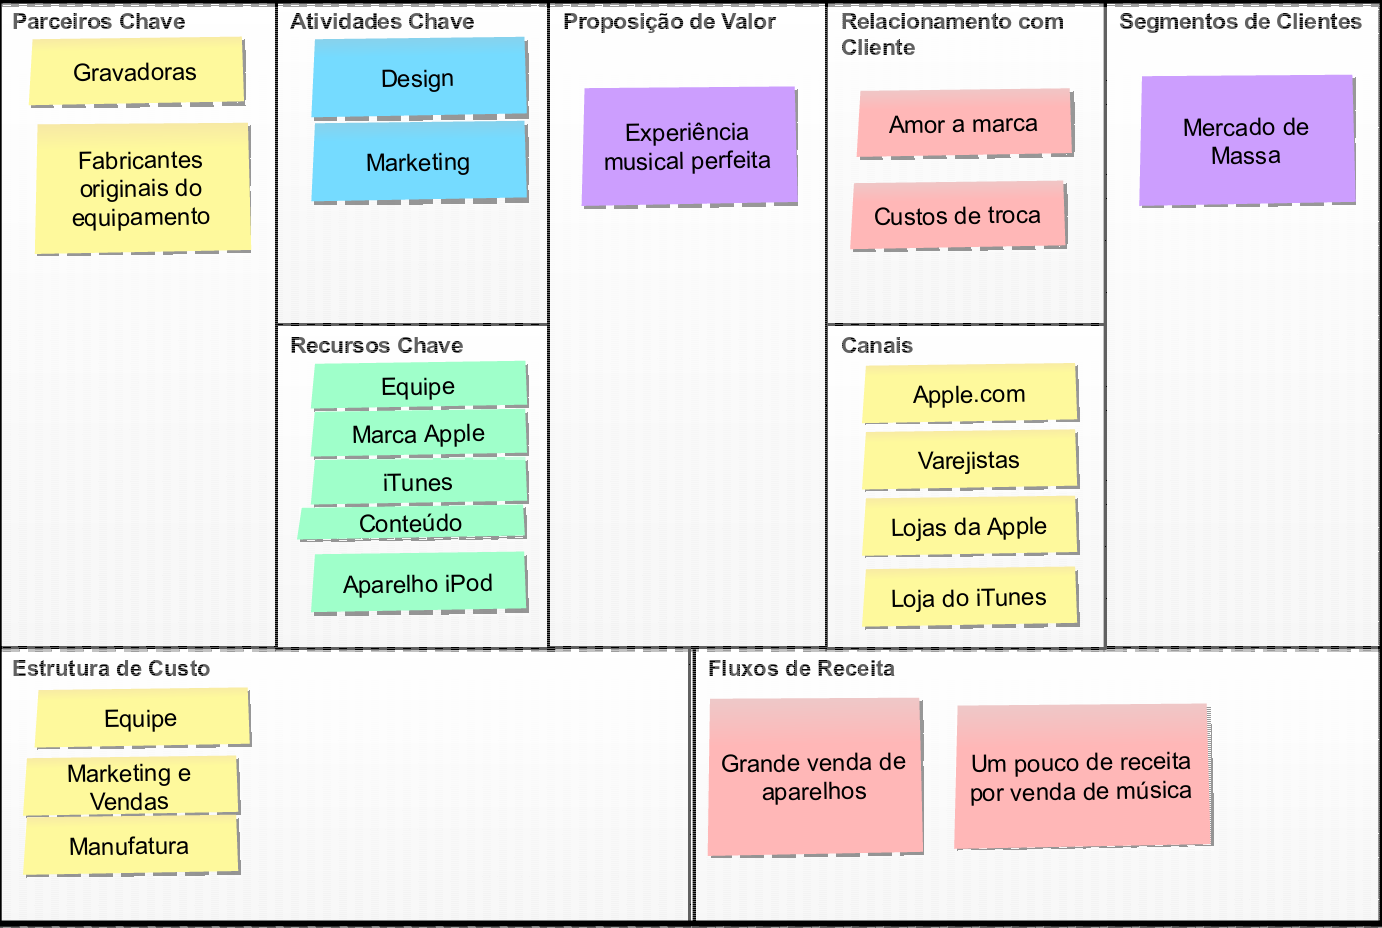
\includegraphics[scale=0.25]{img/canvas_ipod}}
\label{fig:canvas_ipod}
\caption* {Fonte: \citeonline{businessmodel}}
\end{figure}

\subsubsection{Segmento de Clientes}
\label{cha:segmento_de_clientes}
Segundo \citeonline{businessmodel}, o segmento de clientes é o conjunto de clientes ou negócios para o qual a empresa pretende vender seus produtos ou serviços.
Nesse bloco, \citeonline{businessmodel}, propõem que o empreendedor responda as seguintes perguntas:
\begin{itemize}
\item Para quem a empresa está gerando valor?
\item Que problemas os clientes querem que a empresa resolva?
\end{itemize}
Os diferentes tipos de segmentos de clientes são: Mercado de Massa, Mercado de Nicho, Segmentado, Multi lateral.

\citeonline{businessmodel} afirmam que no Mercado de Massa as proposições de valor, canais de distribuição e relacionamentos com clientes são destinados para o consumo de um grande número de pessoas que têm um problema ou uma necessidade comum que exige o cumprimento. Os produtos e serviços que têm como alvo o segmento de mercado de massa são atraentes ou satisfazem as necessidades de uma ampla seção transversal da população.

Segundo \citeonline{businessmodel}, o mercado de nicho se refere a um segmento de clientes com características extremamente definidas e necessidades muito particulares. Este segmento exige e espera um produto altamente customizado, feito sob medida para atender às suas necessidades. Portanto, as propostas de valor, relacionamento com clientes, canais de distribuição estão estreitamente definidos de acordo com as preferências deste segmento de clientes.

Para \citeonline{businessmodel} algumas empresas optam por fornecer produtos e serviços para os segmentos de clientes que podem ter variações muito pequenas em suas necessidades e exigências. A organização cria proposições diferentes valores, canais de distribuição e relacionamento com os clientes de acordo com estas pequenas diferenças nos segmentos de clientes. Um exemplo seria no caso dos bancos de varejo que criam diferentes tipos de contas/produtos de acordo com a renda mensal de cada cliente.

Outro tipo de segmento é o Multilateral. Segundo \citeonline{businessmodel}, quando os segmentos de clientes são dependentes faz sentido para o negócios servir ambas as extremidades da equação. Um exemplo seria um aplicativo para pedir táxis. A empresa criadora do aplicativo precisa satisfazer as necessidades tanto do taxista quanto do passageiro.

\subsubsection{Proposição de Valor}
\label{cha:proposicao_de_valor}
É um conjunto de benefícios, produtos e/ou serviços, que a empresa entrega a um determinado conjunto de clientes, com o objetivo de solucionar problemas ou satisfazer necessidades dos
mesmos. Dessa forma, a proposição de valor é o que torna essa empresa atrativa para
determinado grupo de clientes. \cite{businessmodel}. Em termos simples, uma proposta de valor define porque um cliente escolherá um produto em detrimento de outro, citando o que o produto fornece mais perante seus concorrentes.

Nesse tópico, \citeonline{businessmodel}, propõem que o empreendedor responda as seguintes perguntas:
\begin{itemize}
\item Que problema a empresa está ajudando a resolver?
\item Quais necessidades a empresa está satisfazendo para cada segmento de clientes?
\end{itemize}

\subsubsection{Canais}
\label{cha:canais}
De acordo com \citeonline{businessmodel}, os canais de vendas, comunicação e distribuição são basicamente a interface da empresa com o cliente. Cabe ao empreendedor selecionar os melhores "pontos de contatos" para comunicar o valor proposto e para distribuir e vender seus produtos e serviços.

\subsubsection{Relacionamento com Clientes}
\label{cha:relacionamentos_com_clientes}
Nesse bloco, \citeonline{businessmodel} determinam a natureza das relações que a organização vai desenvolver com os seus vários segmentos de clientes. Uma empresa pode optar por se comunicar com seus clientes através de pessoas ou meios automatizados. As relações com os clientes que uma organização optam por fazer impactam significativamente a experiência geral do cliente.

\subsubsection{Fluxo de Receita}
\label{cha:fluxo_de_receita}
Segundo \citeonline{businessmodel}, as organizações devem precificar o valor que elas oferecem para cada segmento de clientes. Questões como precificação e o modelo de cobrança (aquisição, assinatura, comissão, por exemplo) definem como será o fluxo de receita do modelo.

\subsubsection{Recursos-Chave}
\label{cha:recursos_chave}
Para \citeonline{businessmodel} os Recursos-Chave são os principais insumos que a sua empresa utiliza para criar a sua proposta de valor, servir seus segmentos de clientes e entregar o produto aos clientes. Estas são as coisas mais importantes que a empresa precisa ter para o seu modelo de negócio funcionar.Modelos de negócios são geralmente baseados em uma série de recursos tangíveis e intangíveis. Estes são os principais ativos que a empresa necessita para criar o produto final, e estes geralmente são diferentes dos principais recursos estão sendo utilizados por concorrentes. . Este aspecto desempenha um papel direto em trazer a sua proposta de valor para a vida para o segmento de clientes escolhido e define o mínimo necessário para oferecer valor aos clientes.

\subsubsection{Parcerias-Chave}
\label{cha:parcerias_chave}
De acordo com \citeonline{businessmodel} esse tópico refere-se à rede de fornecedores e parceiros que
tornam o modelo de negócio eficaz. As razões para uma empresa de optar por uma parceria são inumeráveis, mas parcerias saudáveis são fundamentais para tornar o negócio um sucesso ou um
fracasso. Uma empresa pode otimizar a sua utilização de recursos, criar novos fluxos de recursos ou
mitigar os riscos subjacentes às principais decisões de negócios ao assumir um parceiro antes de
iniciar um novo curso de ação. É importante notar aqui que uma organização talvez faça parcerias com
uma série de organizações, por várias razões, mas nem todos os seus relacionamentos serão a chave
para o negócio ser um sucesso.

\subsubsection{Atividades-Chave}
\label{cha:atividades_chave}
Segundo \citeonline{businessmodel}, não faz sentido uma empresa deter todos os recursos e executar todas as atividades por si só. As atividades-chave são as tarefas mais importantes que uma empresa deve realizar, a fim de cumprir a sua finalidade do negócio. Para ser bem sucedida, a empresa deve realizar ações-chave que são ditadas principalmente pelo seu modelo de negócio. Assim como os recursos-chave, as atividades-chave são igualmente cruciais em uma organização para cumprir sua proposta de valor, atingindo seus segmentos de clientes, manter os seus relacionamentos com os clientes e, finalmente, criar fluxos de receitas a longo prazo.

\subsubsection{Estrutura de Custos}
\label{cha:estrutura_de_custos}
Descreve todos os custos incorridos para que o modelo seja praticado. Os custos são definidos a partir das informações reunidas sobre Recursos Chave, Atividades Chave e Parceiros Chave. \cite{businessmodel}

\subsection{Canvas de Proposição de Valor}
\label{cha:canvas_de_proposicao_de_valor}
Enquanto o canvas de modelo de negócio foca em como gerar valor para o negócio, o canvas de proposição de valor foca em gerar valor para o cliente.
\citeonline{valueproposition} criaram um modelo simples para que o empreendedor possa desenvolver uma proposta de valor atraente. Como mostra a \autoref{fig:cross_canvas}, tal modelo pode ser encaixado dentro do canvas de modelo de negócio. 

\begin{figure}[H]
\caption{Como os dois modelos de canvas se relacionam}
\centerline{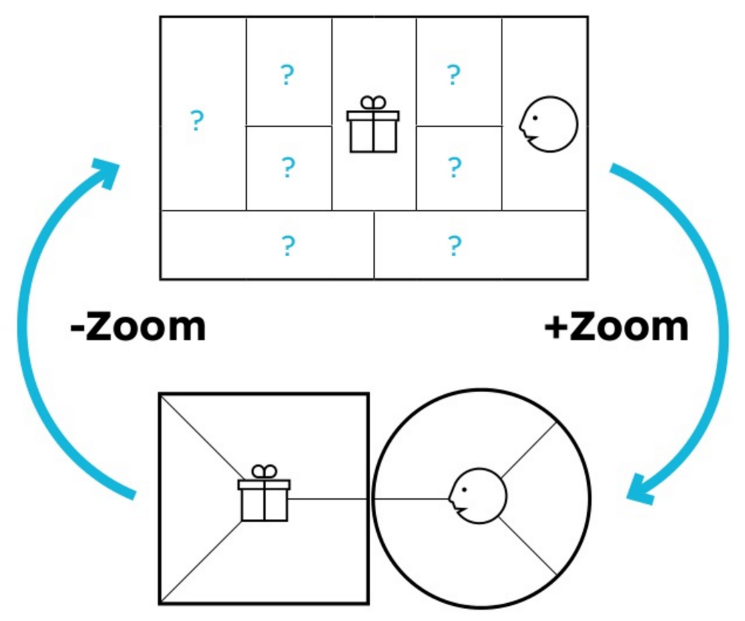
\includegraphics[scale=0.25]{img/cross_canvas}}
\label{fig:cross_canvas}
\caption* {Fonte: \citeonline{valueproposition}}
\end{figure}

O Canvas de Proposição de Valor consiste em dois blocos:
\begin{itemize}
\item Perfil do cliente
\item Mapa de Valor
\item Adequação
\end{itemize}
Que serão detalhados abaixo.

\subsubsection{Perfil do Cliente}
\label{cha:perfil_do_cliente}
Para construir o perfil do cliente, \citeonline{valueproposition}, dividiram esse bloco em três partes:
\begin{itemize}
\item Tarefas do cliente: são o que o cliente está tentando executar no trabalho e na vida.
\item Dores do cliente: são os riscos, dificuldades e obstáculos relacionados com as tarefas do cliente.
\item Ganhos do cliente: são os benefícios que o cliente está desejando. \cite{valueproposition}
\end{itemize}

\subsubsection{Mapa de Valor}
\label{cha:mapa_de_valor}
Para descrever o tipo de valor a empresa pretende entregar para o cliente,\citeonline{valueproposition} também dividiram esse bloco em três partes como mostra a \autoref{fig:canvas_proposicao_de_valor}:
\begin{itemize}
\item Produtos e serviços: uma lista de todos os produtos e serviços na qual a proposição de valor é construída.
\item Aliviadores de dor: uma descrição de como os produtos e serviços da empresa eliminam ou aliviam as Dores do cliente
\item Criadores de ganho: uma descrição de como os produtos e serviços geram Ganhos do cliente. \cite{valueproposition}
\end{itemize}

\begin{figure}[H]
\caption{Canvas de Proposição de Valor}
\centerline{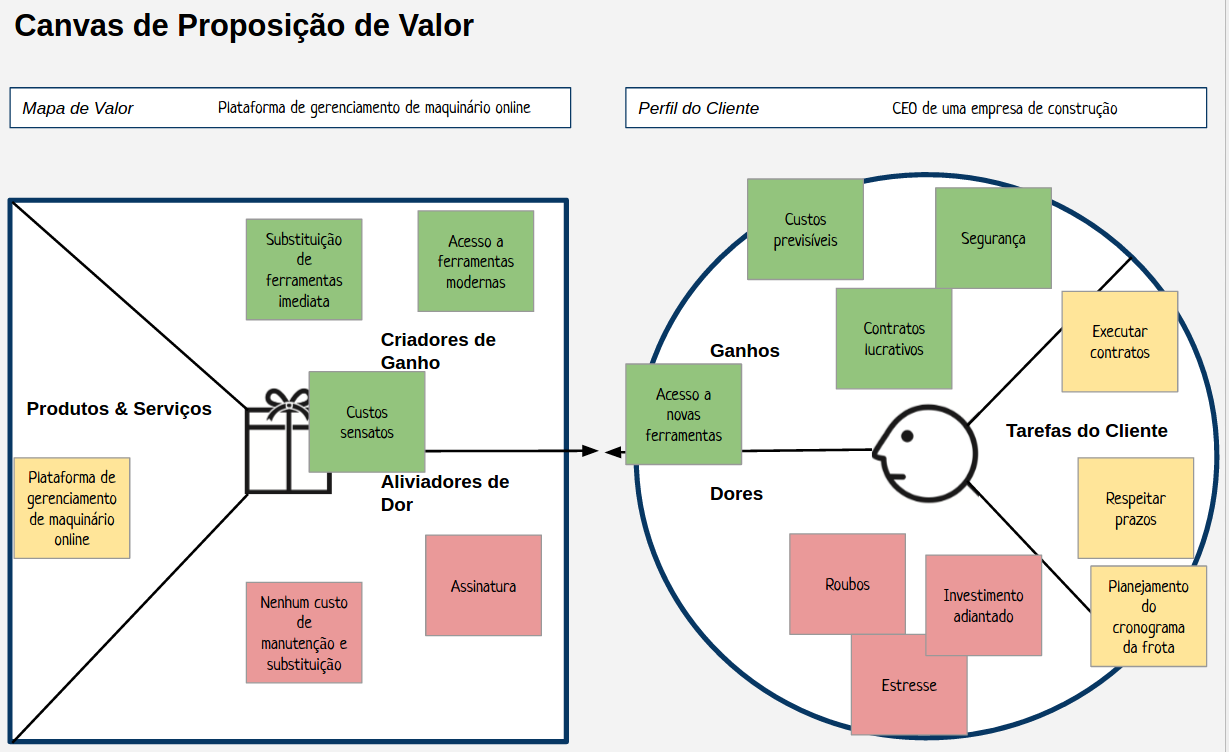
\includegraphics[scale=0.25]{img/canvas_proposicao_de_valor}}
\label{fig:canvas_proposicao_de_valor}
\caption* {Fonte: \citeonline{valueproposition}}
\end{figure}


\subsubsection{Adequação}
\label{cha:adequação}
O objetivo de uma empresa que projeta sua proposição de valor é então atingir a adequação, que ocorre quando a proposição de valor visa tarefas importantes, alivia dores extremas e cria grandes ganhos para com seus clientes. Só é possível verificar se realmente há a adequação com o contato com clientes. \citeonline{valueproposition} sugerem três níveis de adequação:
\begin{itemize}
\item Adequação problema-solução: De acordo com \citeonline{valueproposition}, tal adequação ocorre quando a empresa percebe que os clientes se importam com certas tarefas, dores e benefícios e de que se tem uma proposição de valor que atua em tais itens. Entretanto não há nenhuma evidência de mercado, de que a adequação é real. Nesse momento empresa possui somente intenções de compra normalmente reveladas por reuniões com potenciais clientes.
\item Adequação mercado-produto: Segundo \citeonline{valueproposition}, esse adequação ser atingida apresenta a evidência de que o seu produto/serviço está resolvendo problemas e criando valores reais para os clientes e começa a haver tração do mercado. São observadas as primeiras compras do produto/serviço, confirmando as intenções de aquisição obtidas no estágio anterior. O nível maior de evidências torna possível a verificação de que pelo menos uma porção do mercado enxerga valor real no produto. Para que seja possível atingir essa adequação, todas as suposições do modelo de negócio deverão testadas em um longo processo iterativo envolvendo a interação com potenciais clientes.
\item Adequação do modelo de negócio: Mostra que a empresa tem um modelo de negócio escalável e replicável. Essa adequação é representada por uma somatória de fluxo de receitas maior que a somatória de sua estrutura de custos. Tal lucratividade demonstra que a empresa criou um negócio sustentável. \cite{valueproposition}
\end{itemize}

\begin{figure}[H]
\caption{Adequação da Proposição de Valor}
\centerline{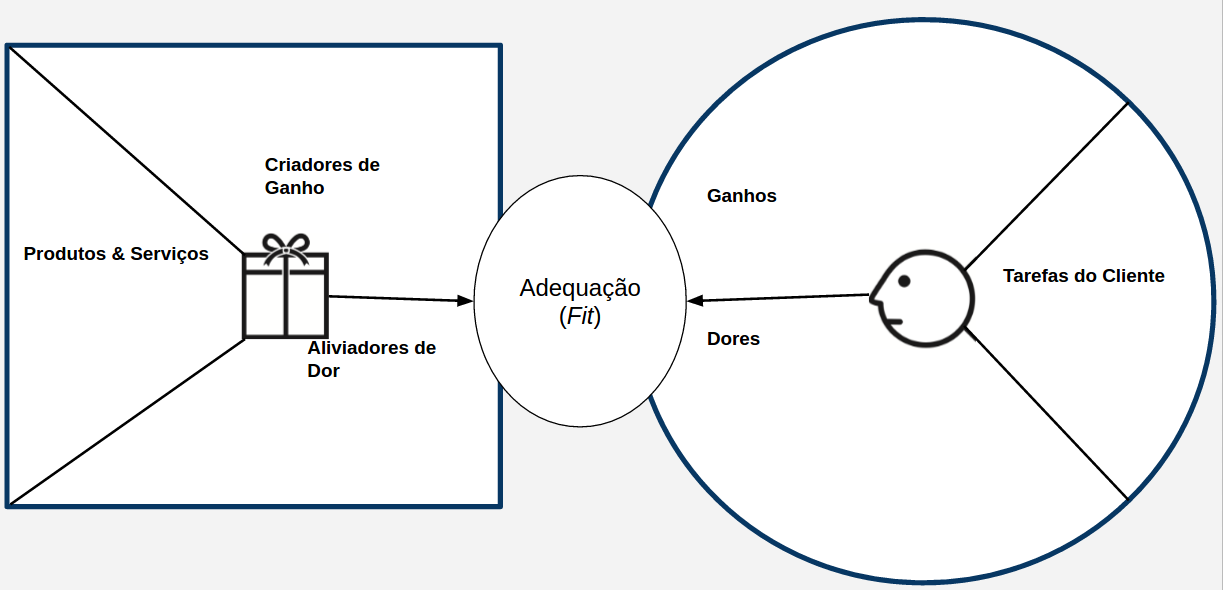
\includegraphics[scale=0.25]{img/value_proposition_fit}}
\label{fig:value_proposition_fit}
\caption* {Fonte: \citeonline{valueproposition}}
\end{figure}